\input sys/inputs.tex

\usepackage[slovak]{babel}

\begin{document}

\bigheading{Kaunterspely}

% \info{task_name}{infile}{outfile}{points}{timelimit}{memlimit}
% leave this values, if you are not interested
\info{counterspells}{stdin}{stdout}{100}{1000 ms}{1 GB}

Baklažán, Žaba, Vlejd, Samko a MišoF si jedného pekného dňa povedali,
že si spolu zahrajú Medžiky. Všetci piati naraz.

Ako sa dalo čakať, jedna hra trvala zrhuba 7 hodín a vzniklo v nej niekoľko
veselých situácií. Na základe jednej z nich vznikla aj táto úloha.

\heading{Úloha}

Vrcholy každého zakoreneného stromu sa dajú jednoznačným spôsobom zafarbiť dvomi
farbami (bielou a čiernou) tak, aby platilo:

\begin{itemize}
\item Vrchol je biely práve vtedy, keď má aspoň jedného čierneho syna.
\end{itemize}

Jednoznačnosť tohto farbenia sa dá ľahko dokázať indukciou. Stromy zafarbené takýmto
spôsobom budeme volať \emph{pekne vyfarbené}.

Vezmeme zakorenený strom obsahujúci jediný čierny vrchol (koreň) a $n$-krát na
ňom urobíme nasledovnú operáciu:

\begin{itemize}
\item $add(v)$ -- Pridáme do stromu nový čierny vrchol ako syna vrcholu $v$. Následne zmeníme farbu
                  niektorých vrcholov tak, aby výsledný strom bol pekne vyfarbený.
\end{itemize}

Pre každú operáciu nás zaujíma, koľkým vrcholom sme počas nej museli zmeniť farbu na opačnú.

\heading{Vstup}

Koreň stromu má číslo $0$, ostatné vrcholy sú očíslované $1, 2, \dots, n$ v poradí, ako ich
pridávame do stromu.

Prvý riadok vstupu obsahuje jedno celé číslo $n$ ($1 \leq n \leq 200\,000$) -- počet operácií
pridania vrcholu.

Nasleduje $n$ riadkov, $i$-ty z nich obsahuje číslo $v_i$ -- číslo otca\footnote{koňa strýka sestry brata} vrcholu pridaného v $i$-tej operácii. Je zaručené, že vrchol $v_i$ pred $i$-tou operáciou
už existuje, teda $v_i < i$.

\heading{Výstup}

Pre každú operáciu (v poradí, ako sa vykonávajú) vypíšte jeden riadok obsahujúci počet vrcholov, ktoré
sme museli počas tejto operácie prefarbiť.

\heading{Podúlohy}

\begin{center}
\begin{tabular}{|l|l|l|l|}
\hline
podúloha & body & maximálne $n$ & iné obmedzenia                  \\ \hline
1       & 20     & $1\,000$      &                                        \\ \hline
2       & 20     & $10\,000$     &                                        \\ \hline
3       & 20     & $100\,000$     &                                        \\ \hline
4       & 20     & $200\,000$    & Hĺbka finálneho stromu bude nanajvýš $100$. \\ \hline
5       & 20     & $200\,000$    &                                        \\ \hline
\end{tabular}
\end{center}

\heading{Príklady}


\sampleIN
5
0
1
2
1
3
\sampleOUT
1
2
3
2
2
\sampleCOMMENT
Situácia po jednotlivých operáciách vyzerá nasledovne (čerstvo prefarbené vrcholy sú vždy zvýraznené):
\sampleEND
\center{
\includegraphics[width=12cm]{img/counterspells}
}
\end{document}
